% arara: mkdir: {target: "out/tex"}
% arara: symlink: {target: "../main.pyg", linkname: "out/main.pyg"}
% arara: pdflatex: {synctex: true, action: nonstopmode, options: "-shell-escape -recorder -file-line-error -output-dir=out"}
\documentclass[a4paper]{article}
\usepackage{etex}

%%%% Math formatting
\usepackage{amsfonts} % Extra fonts for math formatting.
\usepackage{amsmath}
\usepackage{amsthm}
\usepackage{oz}

%%%% Graphical stuff.
\usepackage{array}
\usepackage{tikz}
\usetikzlibrary{shapes,arrows,decorations.pathmorphing,positioning}

%%%% Structural stuff
\usepackage{subcaption}
\usepackage{minted} % Python syntax highlighting!

%%%% Leftanguage and font settings
\usepackage[T1]{fontenc} % Proper output encoding for diacritics, etc.
\usepackage{lmodern} % Quite a nice font.
\usepackage[UKenglish]{babel} % Basic language setting.
\usepackage[babel=true]{microtype} % Nicer looking text.
\usepackage[autostyle]{csquotes} % Better quoting.

%%%% Appearance
\usepackage{titling} % Better control over the title.
\usepackage{booktabs} % High-quality tables.
\usepackage{xcolor} % Easier handling of colors.

%%%% Title, author, etc.
\title{MDP Tutorial}
\author{Dimitri Klimenko}

%%%% Setup for the hyperref package.
\usepackage[bookmarks=true, pdfpagelabels]{hyperref} % Dynamic linking!
\hypersetup{
  pdftitle={\thetitle},
  pdfauthor={\theauthor},
  colorlinks,
  linkcolor={red!50!black},
  citecolor={blue!50!black},
  urlcolor={blue!80!black}
}

\newcommand{\R}{\mathbb{R}}
\newcommand{\expec}[1]{\mathbb{E} \left[{#1}\right]}
\DeclareMathOperator*{\argmin}{arg\,min}
\DeclareMathOperator*{\argmax}{arg\,max}

\newcommand{\stSpace}{\mathcal{S}}
\newcommand{\actSpace}{\mathcal{A}}
\newcommand{\transFunc}{T}
\newcommand{\rewFunc}{R}
\newcommand{\pol}{\pi}
\newcommand{\val}{V}



\newcolumntype{P}{%
>{\rule[-0.6cm]{0pt}{1.5cm}\centering$}p{1cm}<{$}}

\begin{document}

\maketitle

\section{Problem statement}
\begin{figure}[h]
  \centering
  \caption{The environment}
  \label{fig:env}
  \begin{tabular}{|P|P|P|P|}
    \hline
    1 & 2 & 3 & 4 \tabularnewline
    \hline
  \end{tabular}
\end{figure}
A robot navigates in a very simple environment,
as shown in Figure~\ref{fig:env}.
Suppose the robot starts from cell 1 and tries to reach the goal state, which is
cell 4.
At each time step, the robot can attempt to move one cell to the left,
or one cell to the right.
However, due to control error, every time the robot moves,
it has an 80\% chance of ending up in its intended cell and also a 20\%
chance of staying where it is.
If the robot tries to move left from cell 1, it will simply stay in the
same place.
Each attempted move costs the robot 1 utilon,
while reaching the goal gives a reward of 10.

Please model the above navigation problem as an MDP with an infinite horizon and
discount factor $\gamma=0.95$.

\section{MDP model}
Our MDP model is $(\stSpace, \actSpace, \transFunc, \rewFunc, \gamma)$, where
\begin{itemize}
  \item $\stSpace$ is the state space.
  \item $\actSpace$ is the action space.
  \item $\transFunc$ is the transition function.
  \item $\rewFunc$ is the reward function.
  \item $\gamma = 0.95$ is the discount factor.
\end{itemize}

\subsection{State space}
Since the environment is static, we only need one state variable to fully
describe the problem state---the position of the robot.
As such, the state space for this problem can be represented as
\begin{equation*}
  \stSpace = \{s_1, s_2, s_3, s_4\} .
\end{equation*}
As we've said that $s_4$ is a goal state, this implies that the
problem terminates once $s_4$ is reached.
There are multiple ways to do this, but for this problem we will represent
this by making $s_4$ a \emph{terminal state};
after the robot reaches this state it will no longer be able to take any
actions.
For the purposes of an MDP model, this will be equivalent to stating that
all actions will cause it to stay in $s_4$ and give zero reward.
Similarly, since we know that the agent starts in $s_1$, we can call
this state the \emph{initial state}---this would be the root of the tree
if we were using Monte-Carlo Tree Search to solve this problem.

\subsection{Action space}
The robot can only go left or right, so the action space for the problem is
simply
\begin{equation*}
  \actSpace = \{ Left, Right \} .
\end{equation*}

\subsection{Transition function}
The transition function $\transFunc(s, a, s')$ describes the probabilities for
the possible next states $s'$, conditional on the robot being in state $s$
and taking action $a$,
i.e.
\begin{equation*}
\transFunc(s, a, s') = \Pr(S_{t+1}=s' \mid S_t=s, A_t=a) ,
\end{equation*}
where $S_t$ is the state at time $t$, and $A_t$ is the action at time $t$.
For this particular MDP model, we have
\begin{equation*}
T(s_4, Left, s_4) = T(s_4, Right, s_4) = 1
\end{equation*}
since we've stated that the game ends upon reaching $s_4$, so taking
either action from $s_4$ means that you stay there.
We also have
\begin{equation*}
T(s_1, Left, s_1) = 1
\end{equation*}
since moving left from $s_1$ causes us to stay in $s_1$.
Because the robot has an 80\% chance of going where it intended to go,
we have
\begin{gather*}
T(s_2, Left, s_1) =
T(s_3, Left, s_2) =
T(s_1, Right, s_2) =\\
T(s_2, Right, s_3) =
T(s_3, Right, s_4) = 0.8 .
\end{gather*}
Additionally, we have
\begin{gather*}
T(s_2, Left, s_2) =
T(s_3, Left, s_3) =
T(s_1, Right, s_1) =\\
T(s_2, Right, s_2) =
T(s_3, Right, s_3) = 0.2 ,
\end{gather*}
as the robot has a 20\% chance of staying in the same square when it
tries to move to a different one.
For all other transitions, we have
\begin{equation*}
  T(*, *, *) = 0 ,
\end{equation*}
because, for example, the robot can never end up in $s_3$ immediately
after being in $s_1$.

\begin{table}[h!]
  \caption{
    Transition matrix representation of $\transFunc$.
  }
  \label{tab:tm}
  \begin{subtable}{.5\linewidth}
    \centering
    \caption{Transition matrix $P_{Left}$}
    \label{tab:tm_left}
    \begin{tabular}{c|cccc}
            &$s_1$&$s_2$&$s_3$&$s_4$\\
      \hline
      $s_1$ & 1   & 0   & 0   & 0   \\
      $s_2$ & 0.8 & 0.2 & 0   & 0   \\
      $s_3$ & 0   & 0.8 & 0.2 & 0   \\
      $s_4$ & 0   & 0   & 0   & 1
    \end{tabular}
  \end{subtable}
  \begin{subtable}{.5\linewidth}
    \centering
    \caption{Transition matrix $P_{Right}$}
    \label{tab:tm_right}
    \begin{tabular}{c|cccc}
            &$s_1$&$s_2$&$s_3$&$s_4$\\
      \hline
      $s_1$ & 0.2 & 0.8 & 0   & 0   \\
      $s_2$ & 0   & 0.2 & 0.8 & 0   \\
      $s_3$ & 0   & 0   & 0.2 & 0.8 \\
      $s_4$ & 0   & 0   & 0   & 1
    \end{tabular}
  \end{subtable}
\end{table}

An alternative way to represent this information is with
\emph{transition matrices}, one for $Left$, and one for $Right$;
those matrices can be seen in Table~\ref{tab:tm}.
The rows of the transition matrix represent the \emph{current state} $s$,
and the columns represent the \emph{next state} $s'$.
For example, by looking at the cell in the second row and third column in
Table~\ref{tab:tm_right}, we can see that the probability of reaching
$s_3$ when going $Right$ from $s_2$ is 0.8,
i.e. $T(s_2, Right, s_3) = 0.8$.

\subsection{Reward function}
Since we have decided that $s_4$ is a \emph{terminal state}, we are
representing this by having the robot get ``stuck'' in $s_4$ after reaching
it.
This means that we must set the reward for taking actions from $s_4$ to
always be zero, or the robot could simply continue to collect rewards in
$s_4$ forever, as we're using an infinite-horizon MDP.
As such, we must instead give the robot a reward whenever it reaches
$s_4$.
We can't simply give the robot a reward for going $Right$ from $s_3$, as
sometimes the robot stays in $s_3$.
This means that our reward function $R$ needs to take the form
$$R(s, a, s') , $$
which represents the reward for reaching $s'$ after taking action $a$
from state $s$.

As we've said that the robot eternally receives no rewards after $s_4$ is reached,
this means that
\begin{equation*}
  R(s_4, Left, s_4) = R(s_4, Right, s_4) = 0 .
\end{equation*}
The robot is given a reward of 10 reaching $s_4$;
we can also see by inspection of the transition matrices that the only possible
way to reach $s_4$ is by going $Right$ from $s_3$.
Since it costs the robot $1$ utilon every time it moves, we have
\begin{equation*}
  R(s_3, Right, s_4) = 9 ,
\end{equation*}
which incorporates the reward for reaching $s_4$ as well as the move cost.
All other movements of the robot don't reach the goal but still cost one
utilon, so finally we have
\begin{equation*}
  R(*, *, *) = -1
\end{equation*}
for all other transitions.

\subsection{Graphical representation}
This MDP can also be represented via a graph, which can be seen in
Figure~\ref{fig:graph}.
The four blue nodes in the graph represent the various states, $s_1$, $s_2$,
$s_3$ and $s_4$,
while the arrows out of those nodes represent the actions ($Left$ and $Right$)
that can be taken from those states.
The filled black nodes are ``chance nodes'', representing
different possible outcomes due to a random event,
with labels like $p=0.2$ representing the probability $T(s, a, s')$ of
different state transitions.
The integer labels on the ends of the arrows represent the reward function
$R(s, a, s')$, which specifies the reward for reaching state $s'$ after
taking action $a$ from state $s$.

\begin{figure}
  \caption{A graphical representation of the MDP model}
  \label{fig:graph}
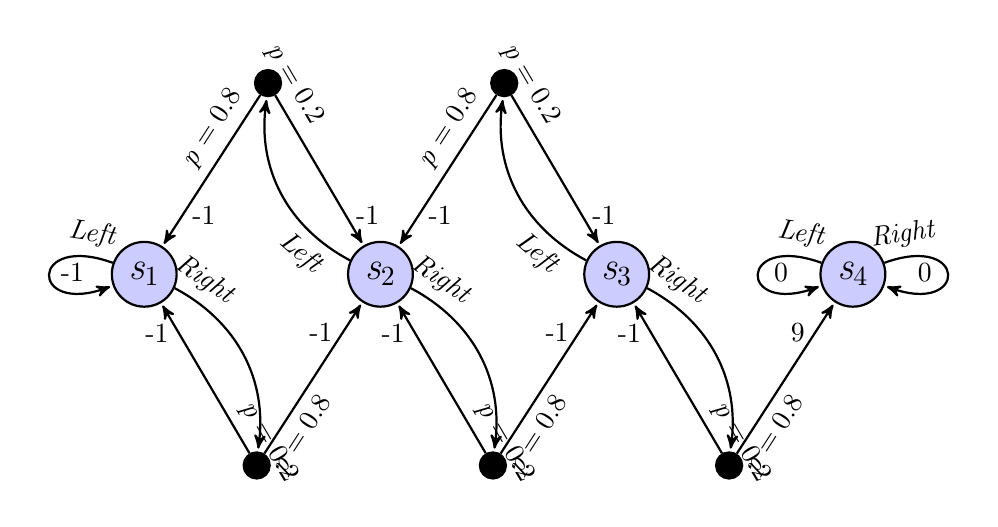
\begin{tikzpicture}[
    ->,>=stealth',shorten >=1pt,auto,node distance=3cm,thick,
  state/.style={circle,fill=blue!20,draw,font=\sffamily\Large\bfseries},
  chance/.style={circle,fill,draw,font=\sffamily\Large\bfseries},
]

  \node[state] (1) {$s_1$};
  \node[state] (2) [right of=1] {$s_2$};
  \node[state] (3) [right of=2] {$s_3$};
  \node[state] (4) [right of=3] {$s_4$};
  \node[chance] (2L) [above left =2cm and 1cm of 2] {};
  \node[chance] (3L) [above left =2cm and 1cm of 3] {};
  \node[chance] (1R) [below right=2cm and 1cm of 1] {};
  \node[chance] (2R) [below right=2cm and 1cm of 2] {};
  \node[chance] (3R) [below right=2cm and 1cm of 3] {};

  \draw [->] (1) to
    [out=160,in=200,looseness=10]
    node[above,sloped,pos=0.1]{$Left$}
    node[above,pos=0.8]{-1}
    (1);

  \draw [->] (2) to
    [bend left=35]
    node[below,sloped,pos=0.2]{$Left$} (2L);
  \draw [->] (2L) to
    node[sloped,pos=0]{$p=0.2$}
    node[right,pos=0.8]{-1}
    (2);
  \draw [->] (2L) to
    node[above,sloped,pos=0.3]{$p=0.8$}
    node[right,pos=0.8]{-1}
    (1);

  \draw [->] (3) to
    [bend left=35]
    node[below,sloped,pos=0.2]{$Left$} (3L);
  \draw [->] (3L) to
    node[sloped,pos=0]{$p=0.2$}
    node[right,pos=0.8]{-1}
    (3);
  \draw [->] (3L) to
    node[above,sloped,pos=0.3]{$p=0.8$}
    node[right,pos=0.8]{-1}
    (2);

  \draw [->] (1) to
    [bend left=35]
    node[sloped,pos=0.1]{$Right$} (1R);
  \draw [->] (1R) to
    node[sloped,pos=0]{$p=0.2$}
    node[left,pos=0.8]{-1}
    (1);
  \draw [->] (1R) to
    node[below,sloped,pos=0.2]{$p=0.8$}
    node[left,pos=0.8]{-1}
    (2);

  \draw [->] (2) to
    [bend left=35]
    node[sloped,pos=0.1]{$Right$} (2R);
  \draw [->] (2R) to
    node[sloped,pos=0]{$p=0.2$}
    node[left,pos=0.8]{-1}
    (2);
  \draw [->] (2R) to
    node[below,sloped,pos=0.2]{$p=0.8$}
    node[left,pos=0.8]{-1}
    (3);

  \draw [->] (3) to
    [bend left=35]
    node[sloped,pos=0.1]{$Right$} (3R);
  \draw [->] (3R) to
    node[sloped,pos=0]{$p=0.2$}
    node[left,pos=0.8]{-1}
    (3);
  \draw [->] (3R) to
    node[below,sloped,pos=0.2]{$p=0.8$}
    node[left,pos=0.8]{9}
    (4);

  \draw [->] (4) to
    [out=20,in=-20,looseness=10]
    node[above,sloped,pos=0.1]{$Right$}
    node[above,pos=0.8]{0}
    (4);

  \draw [->] (4) to
    [out=160,in=200,looseness=10]
    node[above,sloped,pos=0.1]{$Left$}
    node[above,pos=0.8]{0}
    (4);
\end{tikzpicture}
\end{figure}

\section{Policies and value functions}
\subsection{Policies}
A \emph{policy} $\pol : \stSpace \to \actSpace$ is a mapping from states to
actions.
This is the way we describe how the agent in an MDP will act;
in the context of a game we might also call this a \emph{strategy}.

If we associate the states with a specific order, we can also represent a
policy as an ordered list of actions \emph{tuple} that lists one action
for each state.
In this case, the obvious ordering is $(s_1, s_2, s_3, s_4)$,
and so an example policy is
\begin{equation*}
  \pol_L = (Left, Left, Left, Left) .
\end{equation*}
This is clearly not a very good policy because the robot's goal is to
get to the rightmost square, but it's a policy nonetheless!
A policy that's clearly better is
\begin{equation*}
  \pol_R = (Right, Right, Right, Right) ;
\end{equation*}
indeed, this is in fact one of two optimal policies in this MDP,
along with
\begin{equation*}
  \pol_2 = (Right, Right, Right, Left) ;
\end{equation*}

\subsection{Value functions}
A \emph{value function} $\val : \stSpace \to \R$ is a function that associates
each state with a \emph{value}, which is a real number that estimates, for
each state, how valuable it is for us to be in that state.
For example, a relatively silly value function would be
\begin{equation*}
  \val_0(\cdot) \equiv 0
\end{equation*}
which assumes that all states are equally worthless.

\subsection{The value of a policy} \label{ssec:val_pol}
For a given policy $\pol$ we can calculate the value function for
that policy $\val_\pol$ using equations that look like this:
\begin{equation} \label{eq:val_pol}
  \val_\pol(s) = \sum_{s'} T(s, \pol(s), s') \bigg[ R(s, \pol(s), s') + \gamma \val_\pol(s') \bigg] ,
\end{equation}
where $s$ is the current state, $\pol(s)$ is the action that the policy
chooses for that state, and the values $s'$ represent the possible next states.
It's important to note that the value function on the left hand side and right
hand side of the equation is the same one.
Since there many states,
this actually forms a \emph{system of linear equations} that can be solved to
calculate the value of a given policy.
Since there is one equation for each state, and each state has a value,
this is a system of $n$ equations in $n$ unknowns, where $n$ is the number of
states.

Equation~\ref{eq:val_pol} simply represents a calculation of the expected value
over different possibilities for the next state.
This is the sum of two terms:
the value of a given state is the expected value of the immediate reward,
\begin{equation} \label{eq:e_rew}
  \expec{R(s, a, \cdot)} = \sum_{s'} T(s, \pol(s), s') R(s, \pol(s), s')
\end{equation}
added to the discounted expected value of the next state,
\begin{equation}
  \gamma \sum_{s'} T(s, \pol(s), s') \val_\pol(s') .
\end{equation}
If the reward was independent of the next state, we could represent
our reward with a function $R(s, a)$ instead,
with $R(s, a, s') \equiv R(s, a)$.
Consequently, the expected reward over all possible next states
would simply be
\begin{equation*}
  \expec{R(s, \pol(s), \cdot)} \equiv R(s, \pol(s))
\end{equation*}
and Equation~\ref{eq:val_pol} would
simplify to give
\begin{equation} \label{eq:val_rsa}
  \val_\pol(s) = R(s, \pol(s)) + \gamma \sum_{s'} T(s, \pol(s), s') \val_\pol(s') .
\end{equation}

\subsubsection{An example} \label{sssec:val_pol_example}
As an example, we can calculate the value of our not-very-good policy
\begin{equation*}
  \pol_L = (Left, Left, Left, Left) .
\end{equation*}
For convenience, we can turn Equation~\ref{eq:val_pol} into a matrix form.
As you may recall, the transition function can represented by
\emph{transition matrices} (one for each action).
Similarly, the state transitions given a fixed policy can also be described
by a single transition matrix.
Since $\pol_L$ says we should always go left, the appropriate transition
matrix is simply $P_L = P_{Left}$ from Table~\ref{tab:tm_left}, i.e.
\begin{equation*}
  P_L =
  \begin{pmatrix}
      1   & 0   & 0   & 0 \\
      0.8 & 0.2 & 0   & 0 \\
      0   & 0.8 & 0.2 & 0 \\
      0   & 0   & 0   & 1 \\
  \end{pmatrix}
\end{equation*}
Since moving left always has a cost of 1 utilon, we know that the expected
immediate reward will always be -1, except at $s_4$ where the reward
is always zero.
Consequently, we can represent the expected immediate reward by the vector
\begin{equation*}
  \mathbf{r} = \begin{pmatrix}
    -1 \\ -1 \\ -1 \\ 0 \\
  \end{pmatrix} .
\end{equation*}
Using this, we can transform Equation~\ref{eq:val_pol} to the matrix form
\begin{equation} \label{eq:val_matrix}
  \mathbf{v}_L = \mathbf{r} + \gamma P_L \mathbf{v}_L .
\end{equation}
I've switched to the notation $\mathbf{v}_L$ for the value function to
emphasize that it is a \emph{vector} in this equation.
Some basic matrix algebra gives
\begin{equation} \label{eq:val_matrix_simp}
  (I - \gamma P_L) \mathbf{v}_L = \mathbf{r}
\end{equation}
which is simply a system of linear equations in matrix form!
If we substitute the numbers in, we have
\begin{align*}
  \left[
    \begin{pmatrix}
      1 & 0 & 0 & 0 \\
      0 & 1 & 0 & 0 \\
      0 & 0 & 1 & 0 \\
      0 & 0 & 0 & 1 \\
    \end{pmatrix}
    - 0.95
    \begin{pmatrix}
      1   & 0   & 0   & 0 \\
      0.8 & 0.2 & 0   & 0 \\
      0   & 0.8 & 0.2 & 0 \\
      0   & 0   & 0   & 1 \\
    \end{pmatrix}
  \right]
  \mathbf{v}_L &=
  \begin{pmatrix}
    -1 \\ -1 \\ -1 \\ 0 \\
  \end{pmatrix} \\
  \begin{pmatrix}
    0.05  & 0     & 0    & 0    \\
    -0.76 & 0.81  & 0    & 0    \\
    0     & -0.76 & 0.81 & 0    \\
    0     & 0     & 0    & 0.05 \\
  \end{pmatrix}
  \begin{pmatrix}
    \val_L(s_1) \\
    \val_L(s_2) \\
    \val_L(s_3) \\
    \val_L(s_4)
  \end{pmatrix}
  &=
  \begin{pmatrix}
    -1 \\ -1 \\ -1 \\ 0 \\
  \end{pmatrix} .
\end{align*}
If we solve the equations, we get
\begin{gather*}
  \val_L(s_4) = 0 \text{, and} \\
  \val_L(s_1) = \val_L(s_2) = \val_L(s_3) = -20 .
\end{gather*}
This would mean that, from our initial state of $s_1$,
the expected value of our policy $\pol_L$ is -20.
Clearly not a very good policy\dots

\subsection{The one-step best policy for a value function} \label{ssec:one_step}
Just as we calculated the value function for a given policy,
we can start with a value function and work out what the best
policy would be if those values were actually correct.
This is a little weird, because if start with wrong values
and work out a policy for those values that would actually
change what the values would be.
The way we make sense of this idea is that we specifically look
only \emph{one step ahead} in working out which action to take
from every state - this is a \emph{one-step best policy}.

To make this simpler, we introduce the notion of a \emph{Q-value} $Q^*(s, a)$.
The Q-value of a state and action is the value of taking action $a$ from
state $s$, and following an optimal policy therewith.
However, for a one-step best policy we don't necessarily know that our value
function correctly represents the value of an optimal policy,
and we don't necessarily know what the optimal policy is to begin with.
Further detail on the true or optimal Q-value is given in
Section~\ref{ssec:optimal}.
Instead, for our purposes we use a \emph{one-step Q-value estimate}
$\widetilde{Q}_\val$,
which represents the value of taking action $a$ from state $s$ under the
assumption that the given value function $\val$ correctly represents the values
of the subsequent next states.
This estimate is, similarly to Equation~\ref{eq:val_pol}, described by
\begin{equation} \label{eq:q_est}
  \widetilde{Q}_\val(s, a) =  \sum_{s'} T(s, a, s') \bigg[ R(s, a, s') + \gamma \val(s') \bigg] .
\end{equation}
Note that, just as we did for Equation~\ref{eq:val_rsa}, we can simplify this equation in
the case where our reward is completely independent of the next state;
this would result in
\begin{equation} \label{eq:q_est_rsa}
  \widetilde{Q}_\val(s, a) =  R(s, a) + \gamma \sum_{s'} T(s, a, s') \val(s') .
\end{equation}
Now, in order to work out a one-step best policy for a given value function,
we look one step ahead for every state and choose the action that has the
best one-step value for each state.
Consequently, the one-step best policy can be defined like this:
\begin{equation} \label{eq:one_step_pol}
  \widetilde{\pol}_\val(s) = \argmax_a \widetilde{Q}_\val(s, a) = \argmax_a \sum_{s'} T(s, a, s') \bigg[ R(s, a, s') + \gamma \val_\pol(s') \bigg] ,
\end{equation}
which simply states that our policy always takes the action that has the largest
expected value when we look one step ahead with our given value function $\val$.

\subsubsection{An example}
As an example, let's start with a value function $\val_\sigma$
($\sigma$ for silly),
which we will represent by the vector
\begin{equation*}
  \mathbf{v}_\sigma = (1, 0, 0, 0) ,
\end{equation*}
which means that we're assuming that being in cell 1 is worth 1 utilon, whereas
being in any of the other cells is worth 0 utilons.

In order to find the one-step best policy, we first calculate the values
of all the actions from looking one step ahead, which gives us the following:
\begin{gather*}
  \widetilde{Q}_\sigma(s_1, Left)  = -1 + 0.95 \cdot 1 = -0.05 \\
  \widetilde{Q}_\sigma(s_1, Right) = -1 + 0.95 (0.8 \cdot 0 + 0.2 \cdot 1) = -0.81 \\
  \widetilde{Q}_\sigma(s_2, Left)  = -1 + 0.95 (0.8 \cdot 1 + 0.2 \cdot 0) = -0.24 \\
  \widetilde{Q}_\sigma(s_2, Right) = -1 + 0.95 (0.8 \cdot 0 + 0.2 \cdot 0) = -1 \\
  \widetilde{Q}_\sigma(s_3, Left)  = -1 + 0.95 (0.8 \cdot 0 + 0.2 \cdot 0) = -1 \\
  \widetilde{Q}_\sigma(s_3, Right) = 0.8 \cdot (9 + 0.95 \cdot 0) + 0.2 \cdot (-1 + 0.95 \cdot 0) = 7 \\
  \widetilde{Q}_\sigma(s_4, Left)  = 0 + 0.95 \cdot 0 = 0 \\
  \widetilde{Q}_\sigma(s_4, Right) = 0 + 0.95 \cdot 0 = 0 .
\end{gather*}
Note that since the reward is always independent of the next state
(i.e. either -1 or 0)
except when we're in cell 3 and attempt to move right, we've used the simplified
form of Equation~\ref{eq:q_est_rsa} to calculate these q-values.

Now, our one-step best policy is simply a policy that takes the action with the
highest estimated value for each state.
From the above calculations, it's pretty clear that the one-step best action for
$s_1$ and $s_2$ is to go $Left$.
This seems pretty stupid since the robot's goal was supposed to be reaching
$s_4$,
but remember that this is the result of choosing a rather silly value function
that assumed \emph{a priori} that being in $s_1$ was more valuable than being
in $s_2$.
On the other hand, it is quite clear from the above that the one-step best
action for $s_3$ is to go $Right$ for a reward of 7, rather than $Left$
for a reward of -1.
This is because in looking one step ahead from $s_3$ we've seen the immediate
value of potentially reaching the goal.
On the other hand, when we're at $s_4$, we seem to be completely indifferent
between the $Left$ and $Right$ actions, because both of them have an estimated
value of 0.
In that situation it doesn't really matter which one we pick,
so let's pick $Right$.
Consequently, we end up with a one-step best policy
\begin{equation*}
  \widetilde{\pol}_\sigma = (Left, Left, Right, Right) .
\end{equation*}

\subsection{Optimal policies and optimal value functions} \label{ssec:optimal}
Now that we've covered all of the above notions, it's actually rather easy
to define a notion of what it means to have an optimal policy
or an optimal value function.
These two ideas are closely tied together, and they go hand-in-hand with
the notion of a Q-value as we mentioned in the previous section.
The underlying idea is a rather simple one:
for our policy to be \emph{optimal},
it would have to get the absolute maximum possible expected utility
out of every single state we could end up in,
taking into account the fact that it will also continue to maximize
the expected utility from all future states.
Since an MDP involves uncertainty we're necessarily working with
expected utility here---it's not possible to design an agent that
always gets the maximum possible reward every time, because it
might get unlucky.
However, although we can't necessarily maximize our utility, we \emph{can}
ensure that we maximize the \emph{expected utility}.

Fortunately, by a theorem we know that there actually exists an
\emph{optimal value function} $\val^*$, which correctly describes the maximum
expected utility of being in any given state. Additionally, just as we
defined a \emph{Q-value estimate} in Equation~\ref{eq:q_est} using a non-optimal
value function,
we can define the true or optimal Q-value $Q^*$ by using the optimal value
function:
\begin{equation} \label{eq:q}
  Q^*(s, a) = \sum_{s'} T(s, a, s') \bigg[ R(s, a, s') + \gamma \val^*(s') \bigg] .
\end{equation}
As we stated before, the Q-value is the expected value of being in state $s$,
taking action $a$, and then following an optimal policy from that point onward.

If we really knew the optimal value function $\val^*$, it would be very easy for
us to work out the optimal policy.
Since the Q-value is the expected value of taking a given action and behaving
optimally thereafter, this means that all we need to do in order to behave
optimally for the entirety of an MDP is to always select the action with the
highest Q-value from every state!

This is all well and good, but what if we don't know the optimal value function?
Well, using the points we've made above, it's actually rather straightforward
to define an equation---the Bellman optimality equation---that describes the
optimal value function.
Basically, since the action with the highest Q-value from any state must be
optimal, it follows that the value of any state must be equal to the maximum
Q-value!
As such, the Bellman equation looks like this:
\begin{equation} \label{eq:bellman}
  \val^*(s) = \max_a Q^*(s, a) = \max_a \sum_{s'} T(s, a, s') \bigg[ R(s, a, s') + \gamma \val^*(s') \bigg] .
\end{equation}
As you can see, this is just like our very first equation,
Equation~\ref{eq:val_pol}, except that we've now assumed we're always going
to take the action with the best value instead of following a fixed policy.
Crucially, a value function is optimal
\emph{if and only if it satisfies the Bellman equation}.
Additionally, just as we defined a one-step best policy in
Equation~\ref{eq:one_step_pol},
we can define the \emph{optimal policy} as a policy that is a one-step best
policy for the optimal value function!
The equation is simply
\begin{equation} \label{eq:optimal_pol}
  \pol^*(s) = \argmax_a Q^*(s, a) = \argmax_a \sum_{s'} T(s, a, s') \bigg[ R(s, a, s') + \gamma \val^*(s') \bigg] ,
\end{equation}
which is just a different way of saying what we said before---an optimal policy
always selects the action with the highest Q-value from every state.

The interesting thing about the Bellman equation is that it's defined in terms
of only looking \emph{one step ahead},
which might seem unusual at first.
After all, how can we discover an optimal value function by only looking at
a single step?
Well, the key to understanding the Bellman equation is that it is
\emph{recursive}.
The value function is optimal if, after looking one step ahead, you end up
with the same value function again!
Because the definition is recursive, it's a simple matter of mathematical
induction to show that so will looking two steps ahead, three steps ahead,
four steps ahead, and so on to infinity!

In summary, our goal in solving an MDP is to find an \emph{optimal policy}, and
we have some nice equations that such a policy satisfies.
However, we're still left with a major question---how do we \emph{calculate}
an optimal policy?
This is where we bring in our two key methods:
\emph{value iteration} and \emph{policy iteration}.

\section{Value iteration}
\subsection{Explanation}
The basic idea behind value iteration is a rather simple one---let's just use
the Bellman equation directly.
Unfortunately, since it's recursive, it would be pretty hard for us to do
this directly.
Instead, we transform it into an iterative method, in which we continually
apply the Bellman equation to an initial value function.
Each of these steps is called a \emph{Bellman update}.
Moreover, it is guaranteed that as we continue to run our value iteration,
the value function will get closer to and eventually converge to the
optimal value function!
The value iteration algorithm is described by the equation
\begin{equation} \label{eq:val_it}
  \val^{t+1}(s) = \max_a \widetilde{Q}^t(s, a) = \max_a \sum_{s'} T(s, a, s') \bigg[ R(s, a, s') + \gamma \val^t(s') \bigg] ,
\end{equation}
where the superscript $t$ or $t+1$ indicates the current iteration of the
algorithm.
This is basically the Bellman equation, except with the difference that the
left hand side of the equation has $\val^{t+1}$ whereas the right-hand side
has $\widetilde{Q}^t$ and $\val^t$.
In other words, the value function for the next iteration is always received
by using a one-step look-ahead relative to the previous iteration.
That's all there is to it.
Note also that $\widetilde{Q}^t$ is simply the one-step Q-value estimate
for the value function $\val^t$, just like in Equation~\ref{eq:q_est}.

\subsection{Applying it to our robot problem}
So, let's go ahead and try it!
Initially, we will start with
\begin{gather*}
  \val^0(s_1) = \val^0(s_2) = \val^0(s_3) = -1 \\
  \val^0(s_4) = 0 ,
\end{gather*}
where the superscript 0 on the value function indicates that this is
our initial value function, for the 0\ts{th} iteration.

Now, let's work out the one-step Q-value estimates, just like we did
in Section~\ref{ssec:one_step}.
Putting everything into Equation~\ref{eq:q_est} gives
\begin{gather*}
  \widetilde{Q}^0(s_1, Left)  = -1 + 0.95 \cdot -1 = -1.95 \\
  \widetilde{Q}^0(s_1, Right) = -1 + 0.95 (0.8 \cdot -1 + 0.2 \cdot -1) = -1.95 \\
  \widetilde{Q}^0(s_2, Left)  = -1 + 0.95 (0.8 \cdot -1 + 0.2 \cdot -1) = -1.95 \\
  \widetilde{Q}^0(s_2, Right) = -1 + 0.95 (0.8 \cdot -1 + 0.2 \cdot -1) = -1.95 \\
  \widetilde{Q}^0(s_3, Left)  = -1 + 0.95 (0.8 \cdot -1 + 0.2 \cdot -1) = -1.95 \\
  \widetilde{Q}^0(s_3, Right) = 0.8 \cdot (9 + 0.95 \cdot 0) + 0.2 \cdot (-1 + 0.95 \cdot -1) = 6.81 \\
  \widetilde{Q}^0(s_4, Left)  = 0 + 0.95 \cdot 0 = 0 \\
  \widetilde{Q}^0(s_4, Right) = 0 + 0.95 \cdot 0 = 0 .
\end{gather*}
From here, value iteration is pretty straightforward, because we know from
Equation~\ref{eq:val_it} that
\begin{equation*}
  \val^{t+1}(s) = \max_a \widetilde{Q}^t(s, a) .
\end{equation*}
Consequently, the result is
\begin{gather*}
  \val^1(s_1) = -1.95 \\
  \val^1(s_2) = -1.95 \\
  \val^1(s_3) = 6.81 \\
  \val^1(s_4) = 0 .
\end{gather*}
That's one step of value iteration finished!
Now onto the next one:
\begin{gather*}
  \widetilde{Q}^0(s_1, Left)  = -1 + 0.95 \cdot -1.95 = -2.8525 \\
  \widetilde{Q}^0(s_1, Right) = -1 + 0.95 (0.8 \cdot -1.95 + 0.2 \cdot -1.95) = -2.8525 \\
  \widetilde{Q}^0(s_2, Left) = -1 + 0.95 (0.8 \cdot -1.95 + 0.2 \cdot -1.95) = -2.8525 \\
  \widetilde{Q}^0(s_2, Right) = -1 + 0.95 (0.8 \cdot 6.81 + 0.2 \cdot -1.95) = 3.8051 \\
  \widetilde{Q}^0(s_3, Left)  = -1 + 0.95 (0.8 \cdot -1.95 + 0.2 \cdot 6.81) = -1.1881 \\
  \widetilde{Q}^0(s_3, Right) = 0.8 \cdot (9 + 0.95 \cdot 0) + 0.2 \cdot (-1 + 0.95 \cdot 6.81) = 8.2939 \\
  \widetilde{Q}^0(s_4, Left)  = 0 + 0.95 \cdot 0 = 0 \\
  \widetilde{Q}^0(s_4, Right) = 0 + 0.95 \cdot 0 = 0 ,
\end{gather*}
and
\begin{gather*}
  \val^2(s_1) = -2.8525 \\
  \val^2(s_2) = 3.8051 \\
  \val^2(s_3) = 8.2939 \\
  \val^2(s_4) = 0 .
\end{gather*}
One more for good measure:
\begin{gather*}
  \val^3(s_1) = 1.349901 \\
  \val^3(s_2) = 6.026333 \\
  \val^3(s_3) = 8.575841 \\
  \val^3(s_4) = 0 .
\end{gather*}

\subsection{What do we do after we stop iterating?}
OK, so what happens if we stop now, at step 3? What policy would we tell the
robot to use, based on what we've worked out so far?
Well, we can use the same approach we used in
Section~\ref{ssec:one_step}---always recommend the action with the highest
one-step Q-value.
If our value iteration has converged to the true optimal values, or if it's
at least close enough, then the one-step best policy will actually be
a genuine optimal policy!
If we calculated the Q-values for $\val^3$, we would find that the recommended
policy would now be
\begin{equation*}
  \pol^3 = (Right, Right, Right, *) ,
\end{equation*}
which is already optimal!
Note that it doesn't matter whether we go $Left$ or $Right$ from $s_4$,
because the rewards are always 0 regardless.
In fact, we could have stopped with $\val^2$ and we would already have
gotten this result.
Unfortunately, we didn't know this at the time.
Indeed, based on the value iteration algorithm, we don't really have a way
of knowing \emph{for sure} when we've reached a sufficiently accurate
value function to give us an optimal policy,
so we typically just keep iterating until the value function only changes
by a negligible amount from step to step.
Additionally, in the real world, it might take too long for us to reach
a genuine optimal policy, so often we just stop doing value iteration
when we run out of time.

\section{Policy iteration}
\subsection{Explanation}
The basic idea of policy iteration is pretty similar to value iteration,
except that instead of trying to converge a value function towards the
optimal value function, we instead attempt to converge a policy towards
the optimal policy.
For policy iteration, we start with an \emph{initial policy} $\pol^0$,
and we solve Equation~\ref{eq:val_pol} to find the \emph{value function}
for that policy;
using the superscript notation for the time step it looks like this:
\begin{equation} \label{eq:val_pol_it}
  \val^t(s) = \sum_{s'} T(s, \pol^t(s), s') \bigg[ R(s, \pol^t(s), s') + \gamma \val^t(s') \bigg] .
\end{equation}
Just like in Section~\ref{ssec:val_pol}, for a given fixed policy $\pol^t$
this is actually a system of $n$ equations in $n$ unknowns, where $n$
is the number of states.
The unknowns in question are simply the value of each state, e.g.
$\val^t(s_1), \val^t(s_2), \val^t(s_3), \val^t(s_4)$ in our example.

So, once we've worked out the value $\val^t$ of our policy $\pol^t$, what do we do next?
Well, we improve the policy by looking one step ahead, just like we improved our
value function by looking one step ahead in Section~\ref{ssec:one_step}.
Using the superscript notation in Equation~\ref{eq:one_step_pol} gives us this:
\begin{align}
  \pol^{t+1}(s) &= \argmax_a \widetilde{Q}^t(s, a) \nonumber \\
                &= \argmax_a \sum_{s'} T(s, a, s') \bigg[ R(s, a, s') + \gamma \val^t(s') \bigg] . \label{eq:pol_pol_it}
\end{align}
Basically, then, a single iteration of policy iteration consists of repeatedly
applying Equation~\ref{eq:val_pol_it} and Equation~\ref{eq:pol_pol_it}.
In essence, the key to policy iteration is that the policy we use on the next
iteration is the policy we get by looking one step ahead using the value of the
policy from the previous iteration.

One advantage of policy iteration is that it has a rather straightforward
stopping criterion, which follows from the Bellman equation.
In short, if a policy is the one-step best policy for its own value function,
it must be an optimal policy!
This means that we can stop policy iteration once our policy stays the same
from one iteration to the next.

\subsection{Applying it to our robot problem}
Now, let's get down to business, and apply policy iteration to our robot
problem.
We begin with an initial policy
\begin{equation*}
  \pol^0 = (Left, Left, Left, Left) .
\end{equation*}
which says that the robot goes $Left$ in every state.
Now, we apply Equation~\ref{eq:val_pol_it} to solve for $\val^0$.
In fact, we've already done the work for this in
Section~\ref{sssec:val_pol_example}, so we can just re-use our result,
which was
\begin{gather*}
  \val^0(s_4) = 0 \text{, and} \\
  \val^0(s_1) = \val^0(s_2) = \val^0(s_3) = -20 .
\end{gather*}
We can also represent this in vector form,
\begin{equation*}
  \mathbf{v}^0 = \begin{pmatrix}
    -20 \\ -20 \\ -20 \\ 0 \\
  \end{pmatrix} .
\end{equation*}
Now we need to figure out our policy for the next step, $\pol^1$,
using Equation~\ref{eq:one_step_pol}.
In order to do this, we just have to calculate the Q-value estimates
for each action from each state, and pick the action with the highest value.
This is just like when we calculated the Q-values for value iteration,
but this time we're trying to work out the one-step \emph{best action}
$$\argmax_a \widetilde{Q}^t(s, a) $$
rather than the one-step \emph{highest value}
$$\max_a \widetilde{Q}^t(s, a). $$
So, assuming I haven't made an error, the Q-value estimates look like this:
\begin{gather*}
  \widetilde{Q}^0(s_1, Left)  = -1 + 0.95 \cdot -20 = -20 \\
  \widetilde{Q}^0(s_1, Right) = -1 + 0.95 (0.8 \cdot -20 + 0.2 \cdot -20) = -20 \\
  \widetilde{Q}^0(s_2, Left)  = -1 + 0.95 (0.8 \cdot -20 + 0.2 \cdot -20) = -20 \\
  \widetilde{Q}^0(s_2, Right) = -1 + 0.95 (0.8 \cdot -20 + 0.2 \cdot -20) = -20 \\
  \widetilde{Q}^0(s_3, Left)  = -1 + 0.95 (0.8 \cdot -20 + 0.2 \cdot -20) = -20 \\
  \widetilde{Q}^0(s_3, Right) = 0.8 \cdot (9 + 0.95 \cdot 0) + 0.2 \cdot (-1 + 0.95 \cdot -20) = 3.2 \\
  \widetilde{Q}^0(s_4, Left)  = 0 + 0.95 \cdot 0 = 0 \\
  \widetilde{Q}^0(s_4, Right) = 0 + 0.95 \cdot 0 = 0 .
\end{gather*}
Consequently, assuming that we stick to the old policy whenever our
old action is tied for best action with another one,
our next policy for policy iteration is
\begin{gather*}
  \pol^1(s_1) = Left \\
  \pol^1(s_2) = Left \\
  \pol^1(s_3) = Right \\
  \pol^1(s_4) = Left .
\end{gather*}
As you can see, the policy has gotten a little bit smarter;
we've realized that based on what we know so far
going right from $s_3$ is better than going left,
and so we've changed our policy to reflect this.

\subsection{Another step}
Now, let's do another step of policy iteration.
First, we have to work out the value of our new policy, $\pol^1$,
which means solving the system of equations represented by
Equation~\ref{eq:val_pol_it}.
Following our steps from Section~\ref{sssec:val_pol_example},
we start by writing down the transition matrix for our particular
policy.
First, recall our matrices $P_{Left}$ and $P_{Right}$ from
Table~\ref{tab:tm}.
The rows of the matrices represent the transition probabilities
resulting from taking actions $Left$ and $Right$ respectively,
from each of the states.
As such, we can construct our transition matrix for the policy
$\pol^1$ by using the relevant row from $P_{Left}$ or $P_{Right}$
for each of the rows of the matrix $P_1$,
based on the action that $\pol^1$ takes for each state.
We use subscript notation for the transition matrix in order
to avoid confusion with matrix multiplication.
In particular,
\begin{itemize}
  \item the first row of $P_1$ is the first row of $P_{Left}$,
  \item the second row of $P_1$ is the second row of $P_{Left}$,
  \item the third row of $P_1$ is the third row of $P_{Right}$, and
  \item the last row of $P_1$ is the last row of $P_{Left}$.
\end{itemize}
The result is
\begin{equation*}
  P_1 =
  \begin{pmatrix}
      1   & 0   & 0   & 0   \\
      0.8 & 0.2 & 0   & 0   \\
      0   & 0   & 0.2 & 0.8 \\
      0   & 0   & 0   & 1   \\
  \end{pmatrix} .
\end{equation*}
Now we work out the expected immediate reward for each of our states,
$\expec{R(s, \pol^1(s), \cdot)}$.
For $s_1$ and $s_2$ this is clearly -1, and for $s_4$ this is 0.
However, for $s_3$ the expected immediate reward will now be
\begin{equation*}
  \expec{R(s, Right, \cdot)} = 0.8 \cdot 9 + 0.2 \cdot -1 = 7 ,
\end{equation*}
and so we have the reward vector
\begin{equation*}
  \mathbf{r}^1 = \begin{pmatrix}
    -1 \\ -1 \\ 7 \\ 0 \\
  \end{pmatrix} .
\end{equation*}
Now we can use Equation~\ref{eq:val_matrix_simp} to represent our
equations in matrix form, i.e.
\begin{equation}
  (I - \gamma P_1) \mathbf{v}^1 = \mathbf{r}^1 .
\end{equation}
Substituting the values in,
\begin{align*}
  \left[
    \begin{pmatrix}
      1 & 0 & 0 & 0 \\
      0 & 1 & 0 & 0 \\
      0 & 0 & 1 & 0 \\
      0 & 0 & 0 & 1 \\
    \end{pmatrix}
    - 0.95
    \begin{pmatrix}
      1   & 0   & 0   & 0   \\
      0.8 & 0.2 & 0   & 0   \\
      0   & 0   & 0.2 & 0.8 \\
      0   & 0   & 0   & 1   \\
    \end{pmatrix}
  \right]
  \mathbf{v}^1 &=
  \begin{pmatrix}
    -1 \\ -1 \\ 7 \\ 0 \\
  \end{pmatrix} \\
  \begin{pmatrix}
    0.05  & 0     & 0    & 0    \\
    -0.76 & 0.81  & 0    & 0    \\
    0     & 0     & 0.81 & 0.76 \\
    0     & 0     & 0    & 0.05 \\
  \end{pmatrix}
  \mathbf{v}^1 &=
  \begin{pmatrix}
    -1 \\ -1 \\ 7 \\ 0 \\
  \end{pmatrix} ,
\end{align*}
which we can solve to give
\begin{equation*}
  \mathbf{v}^1 = \begin{pmatrix}
    -20 \\ -20 \\ 8.6420 \\ 0 \\
  \end{pmatrix} .
\end{equation*}
Just to make sure we did it correctly, we can use Python to check our
working;
see Listing~\ref{lst:pycon} below for what this looks like!
\clearpage

\begin{listing}[t!]
  \begin{minted}{pycon}
>>> import numpy as np
>>> P1 = np.matrix([[1, 0, 0, 0], [0.8, 0.2, 0, 0],
[0, 0, 0.2, 0.8], [0, 0, 0, 1]])
>>> P1
matrix([[ 1. ,  0. ,  0. ,  0. ],
        [ 0.8,  0.2,  0. ,  0. ],
        [ 0. ,  0. ,  0.2,  0.8],
        [ 0. ,  0. ,  0. ,  1. ]])
>>> r = np.matrix([-1, -1, 7, 0]).transpose()
>>> r
matrix([[-1],
        [-1],
        [ 7],
        [ 0]])
>>> np.linalg.solve(np.identity(4) - 0.95 * P1, r)
matrix([[-20.        ],
        [-20.        ],
        [  8.64197531],
        [  0.        ]]) .
  \end{minted}
  \caption{Python console session, to check our working.}
  \label{lst:pycon}
\end{listing}

Now we calculate Q-values once again, resulting in
\begin{gather*}
  \widetilde{Q}^1(s_1, Left)  = -1 + 0.95 \cdot -20 = -20 \\
  \widetilde{Q}^1(s_1, Right) = -1 + 0.95 (0.8 \cdot -20 + 0.2 \cdot -20) = -20 \\
  \widetilde{Q}^1(s_2, Left)  = -1 + 0.95 (0.8 \cdot -20 + 0.2 \cdot -20) = -20 \\
  \widetilde{Q}^1(s_2, Right) = -1 + 0.95 (0.8 \cdot 8.642 + 0.2 \cdot -20) = 1.768 \\
  \widetilde{Q}^1(s_3, Left)  = -1 + 0.95 (0.8 \cdot -20 + 0.2 \cdot 8.642) = -14.558 \\
  \widetilde{Q}^1(s_3, Right) = 0.8 \cdot (9 + 0.95 \cdot 0) + 0.2 \cdot (-1 + 0.95 \cdot 8.642) = 8.642 \\
  \widetilde{Q}^1(s_4, Left)  = 0 + 0.95 \cdot 0 = 0 \\
  \widetilde{Q}^1(s_4, Right) = 0 + 0.95 \cdot 0 = 0 .
\end{gather*}
Finally, to finish the step, we use these Q-value estimates to derive a new one-step best policy,
which will be
\begin{gather*}
  \pol^2(s_1) = Left \\
  \pol^2(s_2) = Right \\
  \pol^2(s_3) = Right \\
  \pol^2(s_4) = Left .
\end{gather*}

\subsection{Yet another step}
Now that we know how to do it, we might as well keep going.
This time around, we get
\begin{equation*}
  P_2 =
  \begin{pmatrix}
      1   & 0   & 0   & 0   \\
      0   & 0.2 & 0.8 & 0   \\
      0   & 0   & 0.2 & 0.8 \\
      0   & 0   & 0   & 1   \\
  \end{pmatrix} ,
\end{equation*}
and our reward vector is still the same,
\begin{equation*}
  \mathbf{r}^2 = \begin{pmatrix}
    -1 \\ -1 \\ 7 \\ 0 \\
  \end{pmatrix} .
\end{equation*}
Solving for the value function gives
\begin{equation*}
  \mathbf{v}^2 = \begin{pmatrix}
    -20 \\ 6.8740 \\ 8.6420 \\ 0 \\
  \end{pmatrix} ,
\end{equation*}
and the resulting Q-value estimates are
\begin{gather*}
  \widetilde{Q}^2(s_1, Left)  = -1 + 0.95 \cdot -20 = -20 \\
  \widetilde{Q}^2(s_1, Right) = -1 + 0.95 (0.8 \cdot 6.874 + 0.2 \cdot -20) = 0.424 \\
  \widetilde{Q}^2(s_2, Left)  = -1 + 0.95 (0.8 \cdot -20 + 0.2 \cdot 6.874) = -14.894 \\
  \widetilde{Q}^2(s_2, Right) = -1 + 0.95 (0.8 \cdot 8.642 + 0.2 \cdot 6.874) = 6.874 \\
  \widetilde{Q}^2(s_3, Left)  = -1 + 0.95 (0.8 \cdot 6.874 + 0.2 \cdot 8.642) = 5.866 \\
  \widetilde{Q}^2(s_3, Right) = 0.8 \cdot (9 + 0.95 \cdot 0) + 0.2 \cdot (-1 + 0.95 \cdot 8.642) = 8.642 \\
  \widetilde{Q}^2(s_4, Left)  = 0 + 0.95 \cdot 0 = 0 \\
  \widetilde{Q}^2(s_4, Right) = 0 + 0.95 \cdot 0 = 0 .
\end{gather*}
The policy for the next step therefore becomes
\begin{gather*}
  \pol^3(s_1) = Right \\
  \pol^3(s_2) = Right \\
  \pol^3(s_3) = Right \\
  \pol^3(s_4) = Left .
\end{gather*}

\subsection{One more time?}
We said before that the policy $(Right, Right, Right, Left)$ was optimal,
but we haven't really proved that for sure.
So, if we don't know it's optimal and keep running policy iteration,
what happens?

Let's find out.
The new transition matrix is
\begin{equation*}
  P_3 =
  \begin{pmatrix}
      0.2 & 0.8 & 0   & 0   \\
      0   & 0.2 & 0.8 & 0   \\
      0   & 0   & 0.2 & 0.8 \\
      0   & 0   & 0   & 1   \\
  \end{pmatrix} ,
\end{equation*}
and our reward vector is the same once again,
\begin{equation*}
  \mathbf{r}^3 = \begin{pmatrix}
    -1 \\ -1 \\ 7 \\ 0 \\
  \end{pmatrix} .
\end{equation*}
Solving for the value function gives
\begin{equation*}
  \mathbf{v}^3 = \begin{pmatrix}
    5.2151 \\ 6.8740 \\ 8.6420 \\ 0 \\
  \end{pmatrix} ,
\end{equation*}
and the resulting Q-value estimates are
\begin{gather*}
  \widetilde{Q}^3(s_1, Left)  = -1 + 0.95 \cdot 5.215 = 3.954 \\
  \widetilde{Q}^3(s_1, Right) = -1 + 0.95 (0.8 \cdot 6.874 + 0.2 \cdot 5.215) = 5.215 \\
  \widetilde{Q}^3(s_2, Left)  = -1 + 0.95 (0.8 \cdot 5.215 + 0.2 \cdot 6.874) = 4.269 \\
  \widetilde{Q}^3(s_2, Right) = -1 + 0.95 (0.8 \cdot 8.642 + 0.2 \cdot 6.874) = 6.874 \\
  \widetilde{Q}^3(s_3, Left)  = -1 + 0.95 (0.8 \cdot 6.874 + 0.2 \cdot 8.642) = 5.866 \\
  \widetilde{Q}^3(s_3, Right) = 0.8 \cdot (9 + 0.95 \cdot 0) + 0.2 \cdot (-1 + 0.95 \cdot 8.642) = 8.642 \\
  \widetilde{Q}^3(s_4, Left)  = 0 + 0.95 \cdot 0 = 0 \\
  \widetilde{Q}^3(s_4, Right) = 0 + 0.95 \cdot 0 = 0 .
\end{gather*}
The policy for the next step therefore becomes
\begin{gather*}
  \pol^4(s_1) = Right \\
  \pol^4(s_2) = Right \\
  \pol^4(s_3) = Right \\
  \pol^4(s_4) = Left ,
\end{gather*}
which is the same policy we had before.
Policy iteration has converged, so we're definitely finished now.
This means that the policy $\pol^4$ is optimal.

\section{The optimal policy!}
If you look closely at the Q-value estimates $\widetilde{Q}^3$ from policy
iteration,
you'll notice that something very important has happened.
The Q-values satisfy the relationship
\begin{equation*}
  \val^3(s) = \max_a \widetilde{Q}^3(s, a) .
\end{equation*}
For example, the value of state 0 is 5.215, and the maximum Q-value from state
0 is also 5.215.
This means that our value function $\val^3$ satisfies the Bellman optimality
equation (Equation~\ref{eq:bellman}), which said that
\begin{equation*}
  \val^*(s) = \max_a Q^*(s, a) = \max_a \sum_{s'} T(s, a, s') \bigg[ R(s, a, s') + \gamma \val^*(s') \bigg] .
\end{equation*}

In other words, we now know \emph{for sure} that we've found an optimal policy
and the optimal value function!
In summary, we have
\begin{gather*}
  \pol^*(s_1) = Right \\
  \pol^*(s_2) = Right \\
  \pol^*(s_3) = Right \\
  \pol^*(s_4) = Left ,
\end{gather*}
and
\begin{equation*}
  \val^*(s_1) = 5.2151 \\
  \val^*(s_2) = 6.8740 \\
  \val^*(s_3) = 8.6420 \\
  \val^*(s_4) = 0 .
\end{equation*}

Since the value for $s_1$ is 5.2151, we can now confidently say that
the maximum expected utility for the robot is 5.2151 when it starts at
state $s_1$, and that this is precisely the expected utility for
following our optimal policy $\pol^*$.
It's important to note, however, that this is not a unique optimal policy,
as the policy $(Right, Right, Right, Right)$ would also be optimal.
\end{document}
